\documentclass[11pt]{article}
\usepackage{preamble}
\usepackage[]{gset}
\def\week{9}
\def\theproblem{К\week.\arabic{problem}}


\def\FN{\mathcal{N}_f}
\begin{document}
	\setcounter{problem}{0}
	\def\theproblem{Д\week.\arabic{problem}}
	{\textbf{\large Дискретная математика}\hfill \textbf{(Основной поток)}
		
		\medskip %
		
		\textbf{Домашнее задание \week}}
	
	\medskip
	
	\textbf{Дайте обоснованные ответы на следующие вопросы.}
	
	
	\vspace{5mm}
	
	
	\p  Сколько  компонент связности в  лесу на 6 вершинах с 4 рёбрами? Приведите пример такого леса.
	
	Цикломатическое число леса 0.$C$ - цикломатическое число, $v$ - число вершин, $e$ - количество ребер, $c$ - количество компонент связностей. $$C = v - e - c = 0 \Rightarrow c = v - e = 6 - 4 = 2$$
	\[\text{Пример}\]
	\[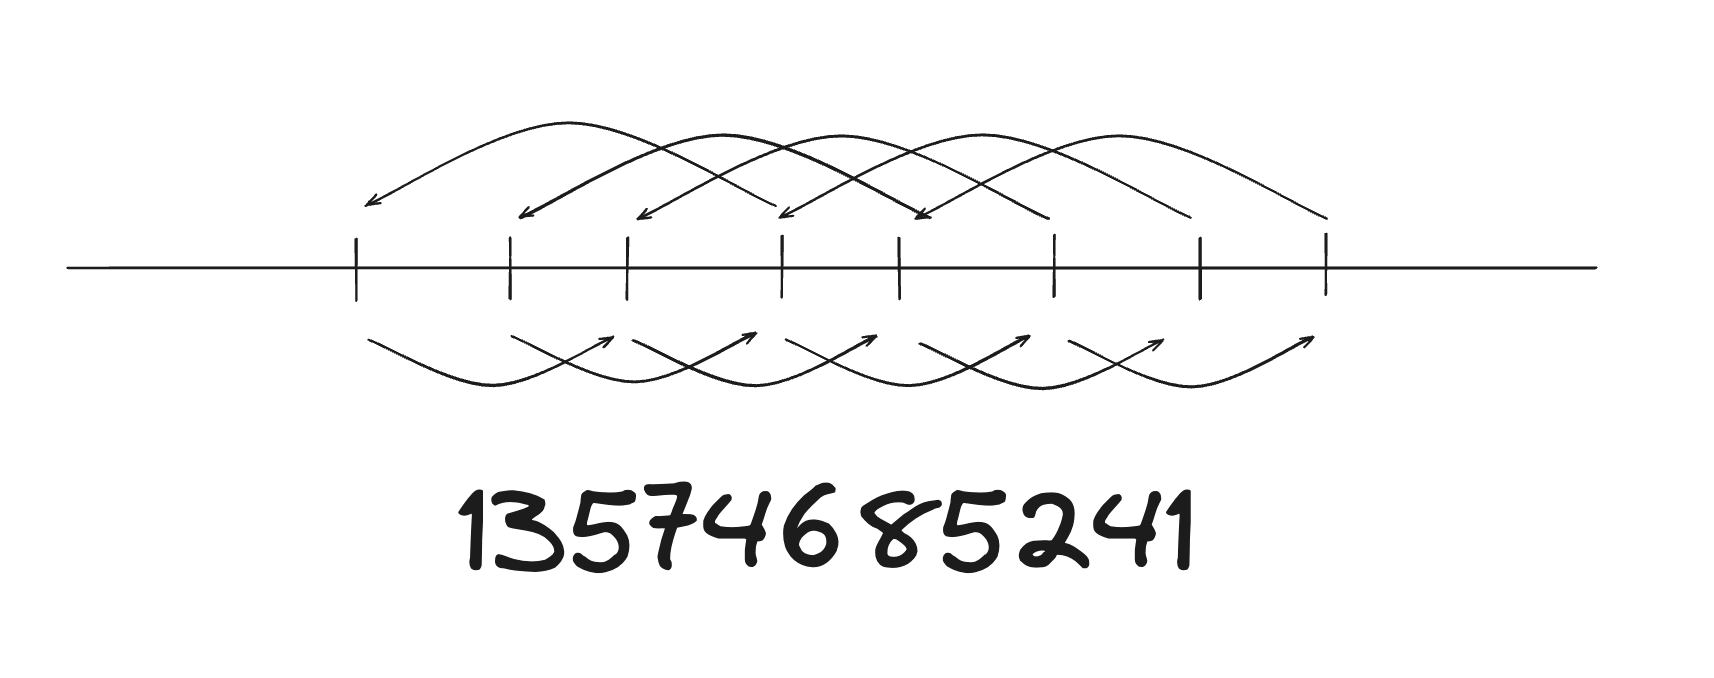
\includegraphics[width=75mm]{img}\]
	
	\p Сколько простых путей может быть в дереве на $n$ вершинах? Укажите все возможные варианты. (Ответ, разумеется, должен быть обоснован.)
	
	Длины 0 может быть ровно $n$ путей. Длины 1 не может быть. Чтобы подсчитать все остальные пути можно выбрать любые две вершины, которые будут соединены, $\frac{n(n - 1)}{2}$ способами. Так как выбрав две вершины получаем ровно 2 простых пути, то всего путей $n(n - 1)$. Получается, что для $n = 1$ ответ $1$, для $n \geq 2$ ответ $n + n(n - 1)$  
	
	\p Найдите наибольшее  количество вершин в связном  графе,  сумма степеней
	вершин в котором равна~20.
	В графе 10 ребер. Логично предположить, что граф дерево, потому что иначе убрав ребро, которое не является мостом, можно "освободить" $\space$ 2 степени вершин и увеличить количество вершин на 1, присоединив новую к любой другой. Получается, что необходимо найти количество вершин в дереве с 10 ребрами. Их 11. \answer{11}
	
 	\p \sp Приведите пример дерева на 14 вершинах, в котором есть ровно две
	вершины степени 6 и нет ни одной вершины степени 2.
	\sp В дереве на 13 вершинах есть ровно две вершины  степени 6. Следует ли из
	этого, что в этом дереве есть вершина степени 2?
	\newpage
	а) 
	\[\text{Пример}\]
	\[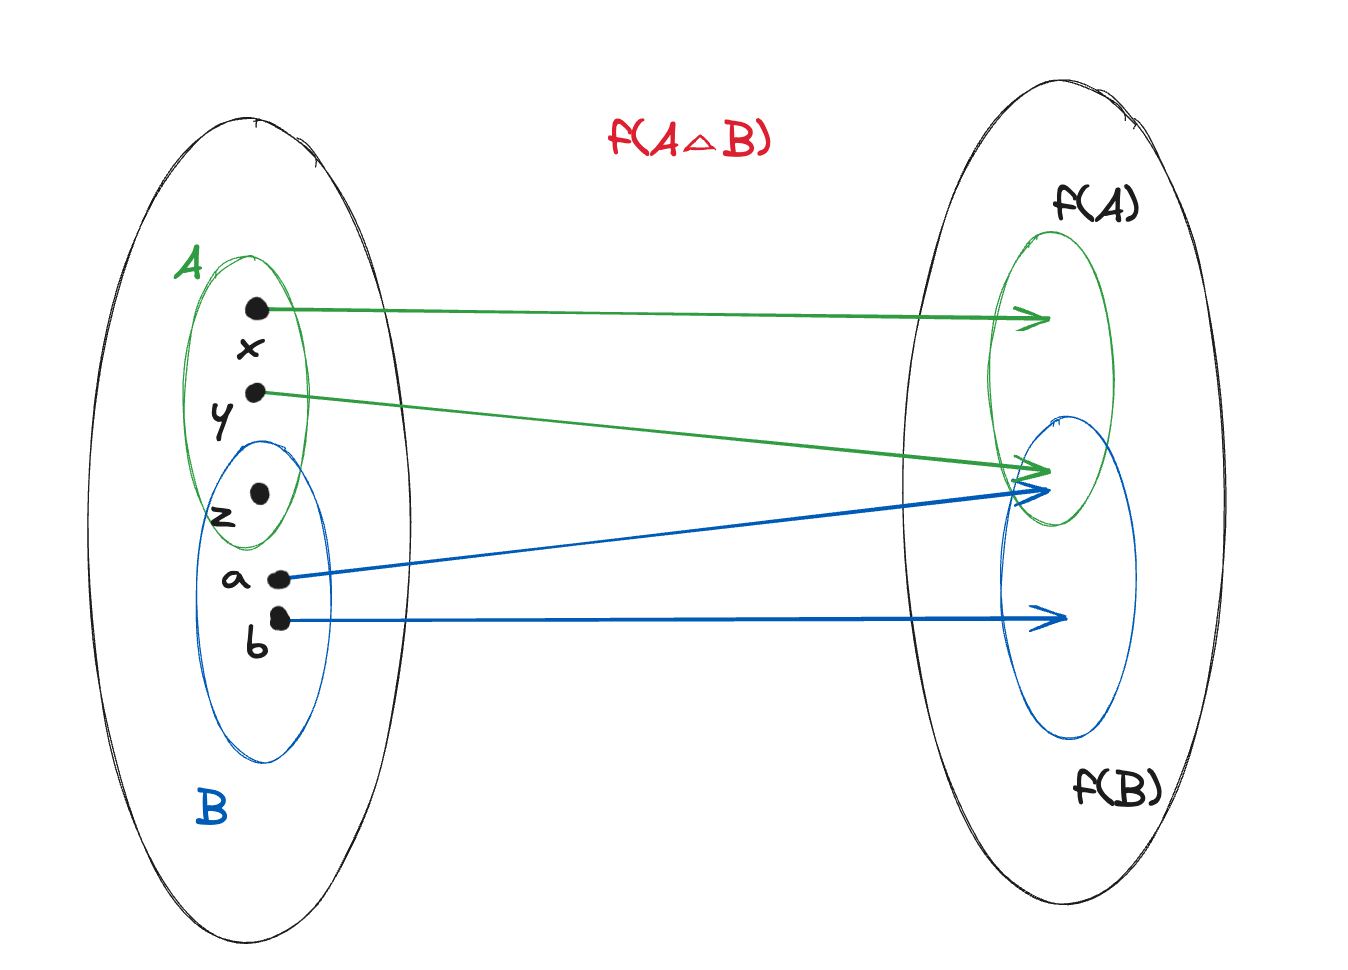
\includegraphics[width=75mm]{img2}\]
	\sspace
	б) В дереве 12 ребер, суммарная степень вершин 24. Сумма степеней 11 вершин кроме 2 степень которых 6 составляет 24 - 12 = 12. Так как степень каждой вершины больше 1, то по принципу Дирихле найдется такая вершина степень которой 2. \answer{Да, следует} 
	
	
	
\end{document}